At the dawn of X-ray crystallography, diffraction data were measured at room temperature, and a full dataset could only be obtained by merging data recorded on several crystals \parencite{kendrewThreeDimensionalModelMyoglobin1958}. Early crystallographers were also particularly interested in elucidating the mechanism of enzymes via crystallography by trapping reaction intermediate states \parencite{hendersonStructureCrystallineAchymotrypsin1970,makinenReactivityCryoenzymologyEnzymes1977}. The rise of cryo-crystallography \parencite{garmanMacromolecularCryocrystallography1997} and high-throughput automated synchrotron \parencite{joachimiakHighthroughputCrystallographyStructural2009} beamlines brought along the era of Structural Genomics, focused on identifying the fold of novel proteins by solving their static structures \parencite{burleyOverviewStructuralGenomics2000,chandoniaImpactStructuralGenomics2006}. The joint effort from a few groups to characterise the dynamical events underlying the mechanism of particular systems \parencite{srajerPhotolysisCarbonMonoxide1996,schotteWatchingProteinIt2003} was unfortunately limited to the study of a few systems. With the combined rise of serial crystallography at XFELs, then synchrotrons \parencite{brandenAdvancesChallengesTimeresolved2021} and the appearance of efficient fold-solving prediction models \parencite{cramerAlphaFold2FutureStructural2021,akdelStructuralBiologyCommunity2022,mccoyImplicationsAlphaFold2Crystallographic2022} have revived the interest in non-standard diffraction experiments probing the dynamics of proteins. 

So far, only a handful of paradigm-defining reactions have been studied by TR-MX, most (not all) are activated by light. Proton pumping by the BR (Section \ref{sec:BR}), signalling by the PYP  (Section \ref{sec:PYP}) and water splitting by the Photosystem II  (Section \ref{sec:Photosystems}) were investigated in an exploratory manner, over several studies, furthering my understanding of fundamental principles governing the dynamics involved in photoreactions. Their design, however, is not suited to investigate more niche or real-life biological systems. 

By carrying out and participating in TR-MX studies, I was able to develop tools directly aimed at solving challenges. In particular, this approach allowed me to bring methodological developments at every stage of a TR-MX experiment, which can be broadly divided into four categories (sample preparation, reaction characterisation, data collection and data analysis), illustrated in Fig. \ref{fig:diagram}, with these discussed in more detail in the following sections. 

\begin{figure}[H]
    \centering
    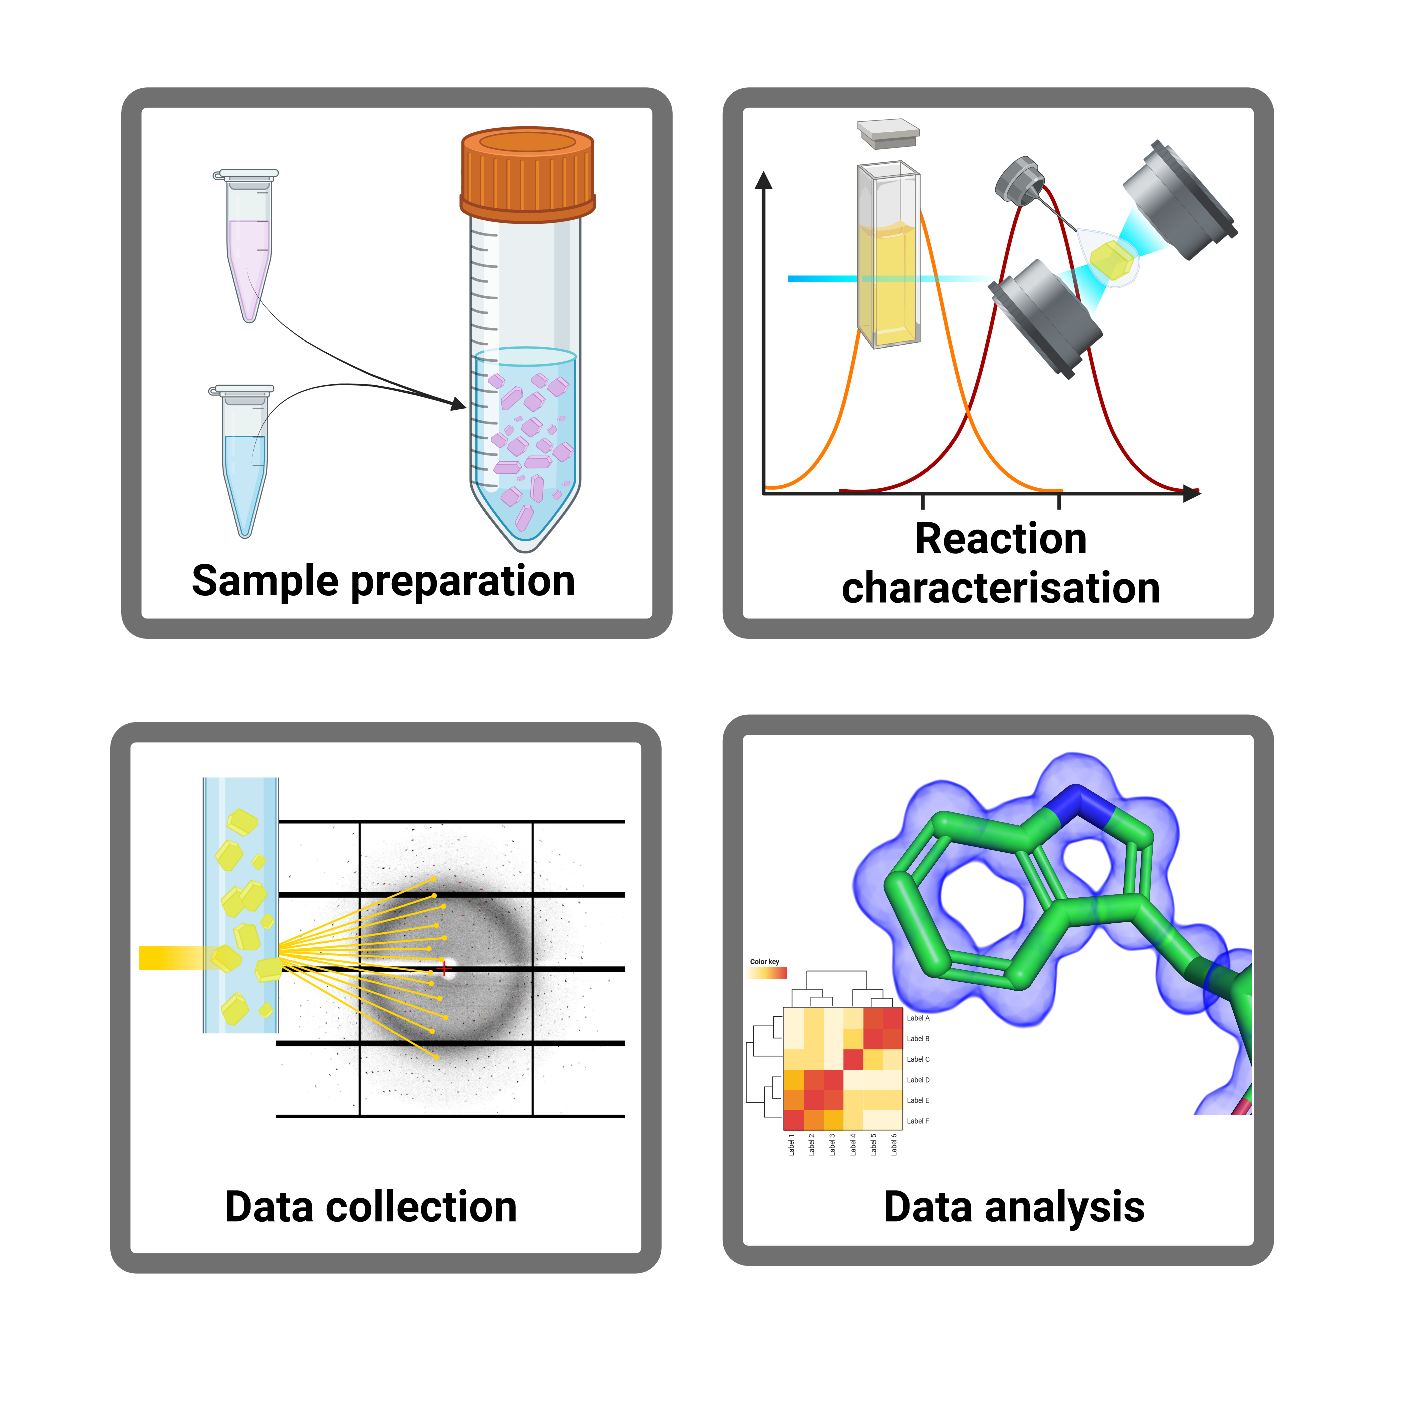
\includegraphics[width=0.8\textwidth]{images/Introduction/TR-MX_diagram.pdf}
    \caption{The four steps needed for a TR-MX experiment}
    \label{fig:diagram}
\end{figure}

\section{Sample preparation: tailoring crystals to specific experiments}

Over the course of this PhD, I prepared samples for experiments with almost opposite requirements: diffusion-based TR-SSX experiment, where crystal size controlled diffusion efficiency, and room-temperature experiments aiming to map slow protein dynamic events, in which any increase in crystal size meant a gain in diffracting power by optimising the X-ray dose repartition over the sample. Through experience, I came up with a set of methods to nudge crystal growth into the direction required by specific experiments. These methods are presented here. 

\subsection{Decreasing the viscosity of a crystal suspension for diffusion-based experiments}
The initial crystallisation condition of T-Cer utilised very viscous precipitants (PEG 8000 or PEG 4000), which was not ideal for diffusion-based experiments. One of the roads explored to improve the sample was to grow the crystal using a salt-based, less viscous precipitant. 

Crystallising a protein with seeds enables the exploitation of the larger metastable growth zone of the crystallisation diagram \parencite{mcphersonCrystallizationProteinsPolyethylene1976, bergforsSeedsCrystals2003}. Crystallisation experiments using seeds are therefore much more tolerant to changes in the precipitation condition. Interestingly, attempts to crystallise T-Cer using (NH\textsubscript{4})\textsubscript{2}SO\textsubscript{4} as a precipitant with seeds made from crystals grown in PEG failed. This is possibly because of the difference in osmotic pressure between the solvent canals of the crystal seeds, and the new crystallisation condition in which they are plunged, which destroys the crystals. In section \ref{sec:ammonium}, I describe a protocol designed to overcome that issue, which leverages the increased tolerance of seeded crystallisation to gradually alter a crystallisation condition over several seeding cycles. 

This protocol allows switching from viscous, polymer-based precipitant in which the majority of protein crystallises, to salt-based precipitant. The viscosity of the crystallisation condition is one of the main factors delaying the diffusion of small molecules in protein crystals \parencite{makinenReactivityCryoenzymologyEnzymes1977}. Being able to grow protein microcrystals in less viscous precipitants could be beneficial to mixing-initiated TR-MX experiments. It would be interesting to see if this protocol can be applied to other, targets, the crystallisation of which is more challenging than T-Cer. 
\vspace{2mm}
A perhaps less extreme version of this idea would be to transfer crystals to increasingly less viscous solutions before they are loaded into the sample environment, with long enough 'resting times' that their solvent canals could be purged of the viscous precipitants.

\subsection{Trimming proteins to maximise their flexibility \textit{in crystallo}}
Controlled proteolysis steps have been widely used to promote crystallisation \parencite{dongSituProteolysisProtein2007,wernimontSituProteolysisGenerate2009,huangSeedingProteaseOptimize2012}. In my group, it has been used to crystallise targets of very high biological interest \parencite{gadellaMScarlet3BrilliantFastmaturing2023}. The rationale of controlled proteolysis is that it removes parts of the protein which are too disordered and could prevent crystallisation, or decrease the order in the crystals. 
\vspace{2mm}
During the T-Cer project, I leveraged limited proteolysis in a counter-intuitive way: I used it to increase the flexibility of the protein in the crystal. By removing the C-terminus of the protein, I partially restored the mobility of the 7\textsuperscript{th} strand, as evidenced by the structure recorded 1 min after a pH drop, in which a noticeable displacement of the strand is observed.  Here, controlled proteolysis removed a segment of the protein which was sticking out of the \textbeta-barrel structure, and into a crystal contact point. This has, to my knowledge, not been done before. Additionally, I simplified the procedure by designing a new construct, equivalent to the state of the protein after the controlled proteolysis step. 
\vspace{2mm}
Taking the idea of increased flexibility \textit{in crystallo} one step further, one could use molecular glues \parencite{engilbergeCrystallophoreVersatileLanthanide2017, alexCalixarenemediatedAssemblySmall2019} to create crystals with looser packings. Possibly, these would allow sufficient mobility to restore the function of proteins which are normally inert \textit{in crystallo}. While that idea has not yet been explored, molecular glues are already used to create supramolecular frameworks \parencite{engilbergeTuningProteinFrameworks2019} or porous crystals \parencite{jonesPorousProteinCrystals2024}.

\subsection{Growing large, ordered crystals}

I have developed a protocol to grow large, well-ordered crystals. Briefly, once the phase diagram of the protein is sufficiently well characterised, seeded crystallisation trials can be set-up so that the drop is maintained in the meta-stable growth zone and never dips into the nucleation zone. For T-Cer, this was achieved by using low concentrations of precipitant and a 1:1:1 ratio of protein solution, mother liquor and milliQ water, respectively. With this protocol, crystal growth can only happen around seed particles, and all the protein in solution in a crystallisation drop is funnelled towards the growth of one or several large crystals. 

Cryoprotecting crystals causes mechanical stress and can decrease their diffracting power. As a solution crystals can also be grown directly in a mother liquor containing their cryoprotectant. For T-Cer, the addition of glycerol slows crystal growth, which prevents the apparition of crystals stacked onto each other. 

\section{Characterising the kinetics of a reaction: how to monitor it, and cross-validate the results of a TR-MX experiment} 
\subsection{Why is it important to compare species identified in solution and \textit{in crystallo}}\label{sec:icOS_interest}
Kinetic crystallography experiments can generate a multitude of diffraction data. For cryo-trapping experiments, significant variations of the experimental strategy (temperature profile, illumination scheme) need to be probed. For TR-SX experiments, many orders of time magnitude have to be explored in order to isolate intermediates of interest. Performing these experiments without prior knowledge could prove to be very time-consuming both for data acquisition and analysis. As discussed in the introduction of this thesis, (Section \ref{sec:potentialbias}), a number of parameters of kinetic experiments such as light fluence for light-driven reactions, humidity level, or photoreduction of cofactors and key amino-acid by the X-ray beam can alter the pathway of a reaction. Further, proteins in the crystalline state, and in crystallising conditions (pH, salinity, temperature) might be far remote from their physiological conditions. For all these reasons, once the experimental parameters have been chosen, it is preferable to cross-validate that the structural species identified in a kinetic crystallography experiment match the species previously identified in the solution. Whether the solution state more accurately represents the physiological state than the crystalline state is a subject of open debate. Nevertheless, the comparison made possible by having access to a technique applicable to proteins in crystals and in solution is valuable. 
\subsection{\textit{in crystallo} UV-vis absorbance spectroscopy to bridge the gap between the crystalline and solution state}
For experiments on coloured proteins, UV-Vis absorption spectroscopy appears to be a suitable complementary technique to rapidly provide information on successful cryo-trapping strategies or time points of particular interest by identifying intermediates with specific spectroscopic signatures \parencite{vonstettenCrystalloOpticalSpectroscopy2015,makitaCombiningOnlineSpectroscopy2023}. A very good example of such a validation is provided in the study of microbial rhodopsin with high-resolution structures of cryo-trapped reaction intermediates. These methods can potentially be extended to non-coloured samples by the use of vibrational spectroscopy: Raman \parencite{buiDirectEvidencePeroxide2014} or infrared \parencite{nomuraShortlivedIntermediateN2O2021,mousDynamicsMechanismLightdriven2022}. 

\begin{figure}[H] %bt!]
    \centering
    \noindent 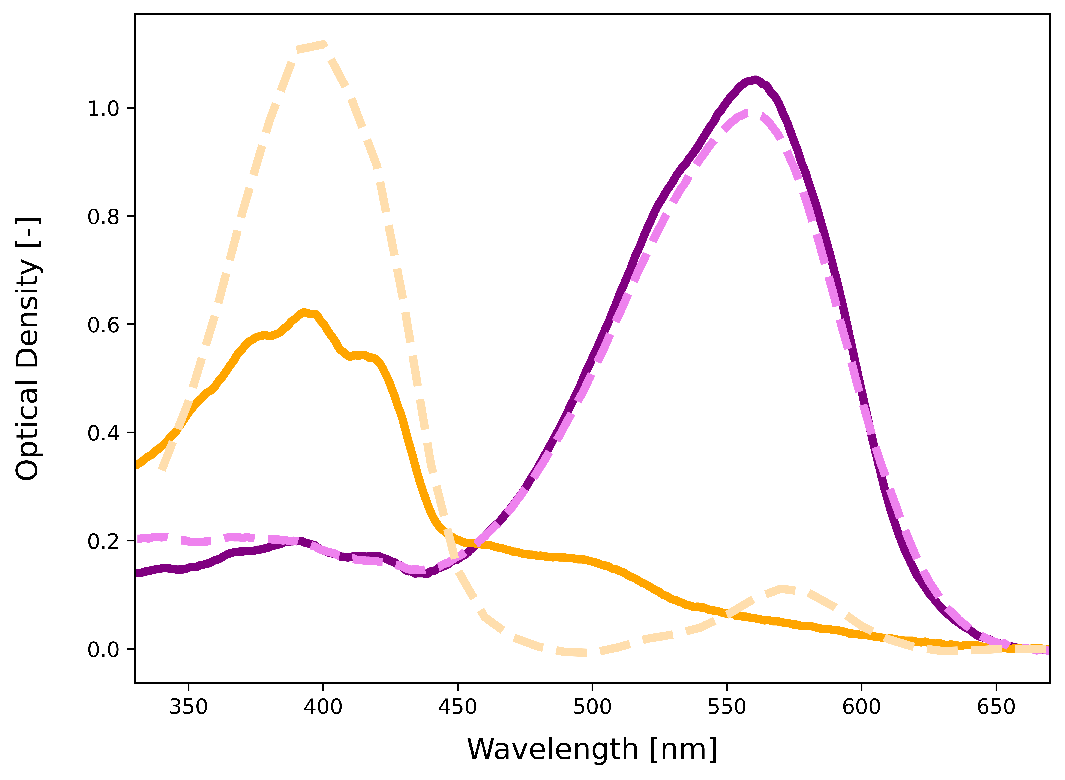
\includegraphics[width=0.7\textwidth]{images/Introduction/Figure2.pdf}
    \hfill
    \caption{\textit{In crystallo} UV-Vis absorption spectra (solid lines) compared with spectra in solution (dashed lines) for the ground state (purple, fuschia) and the cryo-trapped M state (orange, light orange) in the photocycle of BcXeR (data reprised from \cite{kovalevMechanismsInwardTransmembrane2023}). The difference in respective peak heights between the solution and crystal M-state spectra may be due to a polarization effect of the crystal.}
    \label{fig:Figure2}
\end{figure}

\subsection{Making \textit{in crystallo} UV-vis absorption spectroscopy more accessible to unfamiliar users}

To pair the species of T-Cer identified \textit{in crystallo} with the species derived from the initial time-resolved in-solution spectroscopy experiment, I have had to compare many crystals of different sizes and shapes. It is the need for a workflow of spectroscopic data correction which spearheaded the development of the \textit{ic}OS toolbox (Chapter \ref{chap:toolbox}). The set of tools developed was later encased in a graphical interface so that users of the \textit{ic}OS Lab instruments, and of beamline BM07-FIP2 could process their data without the need for my supervision. The toolbox was used in every TR-MX project described in this thesis (Part \ref{part:T-Cer}, Chapters \ref{chap:slowprot}, \ref{chap:CraCRY_TR-SFX_1}, \ref{chap:TR-icOS}, \ref{chap:online-microspec}).

It is now commissioned and accessible for external users, as evidenced by the recent publication of a study in which it was used for baseline correction \parencite{roseSpectroscopicallyValidatedPHdependent2024}. 


\section{Data collection: TR-SSX vs kinetic crystallography}

\subsection{What to do when time-resolved experiments are not possible?}
I first attempted to characterise the reaction of a variant of the Cerulean fluorescent protein, named Twist-Cerulean (T-Cer). The fluorescence of T-Cer is more sensitive to pH variations than that of Cerulean. Additionally, the chromophore of T-Cer adopts a novel configuration at acidic pH. If the characteristics of this protein at acidic pH, as well as the mechanism allowing the conversion from one configuration to the other, are better understood, T-Cer could serve as a paradigm for a pH sensor. This is why I attempted to characterise the mechanism underlying the isomerisation of the chromophore of T-Cer with a TR-SSX approach where the isomerisation would be initiated by mixing crystals grown close to physiological pH with an acidic solution. 
\vspace{2mm}

Unfortunately, I soon realised that the \textit{in crystallo} dynamics of T-Cer significantly differ from its in-solution dynamics. In particular, the movements of an entire strand (7\textsuperscript{th} strand of the \textbeta-barrel structure of T-Cer, coloured orange in Fig. \ref{fig:overall}) appear to be significantly inhibited \textit{in crystallo}, while this strand is particularly mobile in solution \parencite{lelimousinIntrinsicDynamicsECFP2009}. 

Because of the rigidity of that strand \textit{in crystallo}, the isomerisation reaction, which occurs within 80 ms in solution, is prohibited \textit{in crystallo} (it takes several weeks to occur). 

In response to this obstacle, I first leveraged limited proteolysis, then a truncated construct and finally a new, less viscous, crystallisation condition of the protein, to increase the flexibility of this strand \textit{in crystallo}. While these improvements were not enough to allow the isomerisation to occur on the same time scale \textit{in crystallo} as in solution, they did allow it to take place \textit{in crystallo} over < 200 s, so that I could trap crystals while the isomerisation was occurring, by cryo-cooling them at various delays after a pH had been initiated by soaking. Comparing \textit{in crystallo} and in solution UV-vis absorption spectra, I were able to validate that the sequence of events that I derived from high-resolution structures from crystals obtained at various pH accurately reproduced the events triggered by a pH drop in my soaked crystals. Finally, I designed a variant of T-Cer in which a bulky amino acid side chain was removed to allow the chromophore to isomerise regardless of the mobility of the 7\textsuperscript{th} strand. Characterising this variant with high-resolution structures from crystals obtained at acidic and physiological pH revealed that with the reduced steric hindrance, its chromophore does isomerise, but adopts a different configuration at acidic pH than that of T-Cer. 

The role of the N-terminal section of the 7\textsuperscript{th} strand has been extensively studied in my group. Conversely, the role of the C-terminal end of the strand, where the bulky side chain is located, in controlling the conformation of the chromophore by pushing it against residues capable of stabilising it in an H-bond network was not identified until these kinetic and TR-SSX experiments were carried out.

\vspace{2mm}

The methodological novelty brought during the T-Cer was to circumvent the impossibility of recording time-resolved data by recording atomic-resolution static structures, using kinetic crystallography approaches on large crystals and cross-validation with UV-vis absorption spectroscopy. 

\subsection{Probing slow protein dynamics with room-temperature rotation data collection}

The characterisation of the decay of the photoadduct of LOV2 relied on a novel TR-MX scheme, during which an illuminated steady state was populated in the crystals. The decay was probed by recording oscillation datasets at various delays after the illumination had ceased. In TR-SX experiments, the size of the crystals is limited by the penetration depth of the actinic pump light source. Here, the illuminated state was populated with a long illumination (1 min) compared to the time needed for the light-state to be achieved after photo-excitation (\textasciitilde 3 \textmu s, \cite{kasaharaPhotochemicalPropertiesFlavin2002}), which means the entire crystal could be converted. Therefore, this method can make use of large crystals. The increase in volume probed by the X-ray beam means an increase in diffracting power. As this experiment was performed at a microfocus beamline, several datasets could be recorded on the same, large crystal, increasing the throughput.

This method is particularly suited to study systems relaxing from a metastable energy state, that can be populated over time. The decay mechanisms of photosensors are an interesting example of such systems and have not been explored thus far. Yet, the decay mechanism of a photosensor is central to its mechanism, as it regulates the lifetime of its signalling state. 

This method will also be useful to characterise reactions which occur much slower than the diffusion rate of their substrate, for instance, thermophilic enzyme catalysis at room temperature. But this is not limited to enzyme catalysis. The room-temperature soaking experiment performed on T-Cer, produced remarkable results, it could thus be extended into a more systematic sampling of time after a crystal has been delivered an acid, for instance with a nanolitre liquid dispenser. 

Finally, this method can be used to probe reactions which can be homogeneously initiated into a crystal, such as a temperature jump resulting from the pulse of an infrared laser \parencite{wolffMappingProteinDynamics2023}, or the response to an electric field applied to a crystal \parencite{hekstraElectricfieldstimulatedProteinMechanics2016}. 

\subsection{Monitoring the rise of steady-states with the TR-SOX method}

In order to decipher the mechanism leading to the apparition of the signalling state of CraCRY, I have brought several improvements to the TR-SOX methodology, namely, delaying the start of the illumination so that a few images could be recorded on the ground state of the protein. This provides a reference dataset obtained from the same crystals as the time-resolved datasets. 

A major shortcoming was met: the rise of radiation damage towards the end of the series limits the interpretation of the data. This can be addressed for future experiments in two ways: (1) helical data collection across the crystal volume would better ensure that the dose increment remains limited over the course of the data collection. (2) Recording a second series, for which the start of the illumination occurs before the start of data collection will ensure that the first (highest quality) images correspond to longer time-delays. 

Finally, the TR-SOX technique could be adapted to study diffusion-driven reactions, by replacing the actinic illumination with the substrate delivery, the rise of the rate-limiting step of the reaction could then be observed. 
\vspace{2mm}
Of course, the TR-SOX methodology will only ever be able to record the rise of a steady-state population (and eventual decay of intermediate states populations), but the oversampling of the time axis provided as a tradeoff can be utilised by deconvoluting analysis schemes to identify and separate the populations present in the crystal at all times. 

\section{Data analysis: extracting the most from TR-MX data, but no more}

\subsection{SVD analysis: towards quality metrics for each singular vector}

SVD is a powerful analysis tool for difference electron density maps, which allowed me to provide meaningful contributions to the analysis of TR-MX data despite my initially limited knowledge of protein systems studied. It has a major drawback: the choice of the number of meaningful singular vectors produced by the decomposition may be considered subjective. As a solution, I have proposed to integrate the difference electron density of the experimental maps over a region of interest and compare it to the integrated difference electron density in maps reconstructed using only the singular vectors deemed meaningful by the user. If the trend of integrated electron density of the experimental maps is reproduced by the reconstructed maps, then the chosen singular vectors are sufficient to explain the events happening over the region of interest. 

\vspace{2mm}

To go further, one could imagine calculating the average correlation coefficient between the electron density values in voxels of the experimental maps, and in the corresponding voxels of the reconstructed map. This correlation coefficient could be used as a metric revealing how much information is added by each additional singular vector. A cutoff could be defined above which the information added is not sufficient, providing an objective manner of choosing how much singular vectors are 'meaningful'. 

\subsection{SVD analysis benefits from the oversampling of the time-axis}

In TR-SFX pump-probe experiments, each additional recorded time point requires a significant amount of sample and beamtime. As a consequence, most TR-SFX experimenters carefully choose in advance a set of delays after the pump at which they will probe a chemical reaction \parencite{barendsSerialFemtosecondCrystallography2022}. They aim to isolate as best as possible a single reaction intermediate in each recorded dataset. The TR-SOX methodology operates very differently: it samples the build up of a steady state under constant excitation. In doing so, it over-samples the time course of the reaction, which increases the likelihood that a given reaction intermediate is present in a great number of time points. As a drawback, because the TR-SOX uses large crystals, the activation of molecules is not homogeneous throughout the crystal (this is beautifully illustrated in the first supporting video material of \cite{aumonierMillisecondTimeresolvedSerial2020}). Both these elements - oversampling of the time course at the cost of a mixture of states - render this data especially suitable to the SVD analysis utilised in Chapters \ref{chap:MmCPDII} and \ref{chap:CraCRY_TR-SFX_1}. Indeed, SVD greatly benefits from oversampling, the higher the number of datasets decomposed, the more meaningful the produced components are \parencite{henrySingularValueDecomposition1992}, and SVD can deconvolute the mixture of states present in each dataset \parencite{schmidtApplicationSingularValue2003}. 

\section{Consideration on the choice of experimental procedure}

\subsection{Interest of cryo-trapping studies}

Compared with cryo-trapping, time-resolved crystallography appears to be the better-suited approach to probe a reaction since the conditions are closer to the physiological conditions. However, these experiments, which are most often performed with SX, are challenging in terms of sample quantity, experimental knowhow (particularly the control of laser fluence) and diffraction data processing \parencite{barendsSerialFemtosecondCrystallography2022,barendsInfluencePumpLaser2024,bertrandStructuralEffectsHigh2024}, see section Section \ref{sec:dataprocan}. Also, diffraction resolution is often limited at room temperature. Cryo-trapping methods potentially imply a number of drawbacks: flash cooling and cryoprotection artefacts (for trigger-freeze strategies), altered conformational landscape (for freeze-trigger strategies), specific radiation damage (for synchrotron experiments) and limited time resolution, which is dictated by the flash-cooling time, which is just below 1 ms in the best case for microcrystals \parencite{clingerMillisecondMixandquenchCrystallography2021}. However, they do benefit from three significant advantages: (i) production of diffraction data usually at much higher resolution than at room temperature, (ii) ease of diffraction data analysis (for the single-crystal case) and (iii) potentially permitting the accumulation of higher intermediate-state occupancy. The latter can help to overcome the main limitation in kinetic crystallography, which is the difficulty of identifying the structural features of a poorly populated intermediate state, especially when this difficulty is aggravated by non-isomorphism between crystals. While keeping in mind the limitations of cryo-trapping, high-resolution intermediate-state structures can be used to interpret lower-resolution data obtained at room temperature. One final recommendation to navigate between time-resolved approaches and the many cryo-trapping approaches is to perform characterization experiments at various temperatures and with different light excitation schemes (light-source type, wavelength peak or range, duration), possibly via an optical spectroscopy technique applied directly to the crystals prior to diffraction experiments. This would allow researchers to identify the best experimental conditions that induce specific spectroscopic signature changes and thus are most likely to cause specific structural changes.


\subsection{Synchrotron or XFEL}

Applications for XFEL beamtime are highly competitive owing to the small number of facilities that are present around the world. Beamtime for TR-SSX experiments will start to propagate in due course with the emergence of upgraded synchrotrons and beamlines which will allow these types of experiments. One limitation of TR-SSX will be that it is reserved to probing timescales of microseconds and above. At the same time, TR-SFX will continue to enable timescales starting at hundreds of femtoseconds to be probed. However, most enzymes have a turnover in the millisecond-to-second range \parencite{bar-evenModeratelyEfficientEnzyme2011}, making them adequate targets for TR-SSX experiments. This is especially true for mixing experiments, where small-molecule diffusion into crystals will always exceed microseconds and thus is well suited for TR-SSX. As a final point, specific radiation damage does not appear to be a major issue in TR-SSX experiments; however, experiments on particularly radiosensitive samples may still prove to be challenging, for which TR-SFX would continue to be the safer option.